

\begin{frame}[ctb!]
\frametitle{LLNL Model Thermal Conductivity Sensitivity}

\begin{figure}[htbp!]
\begin{center}
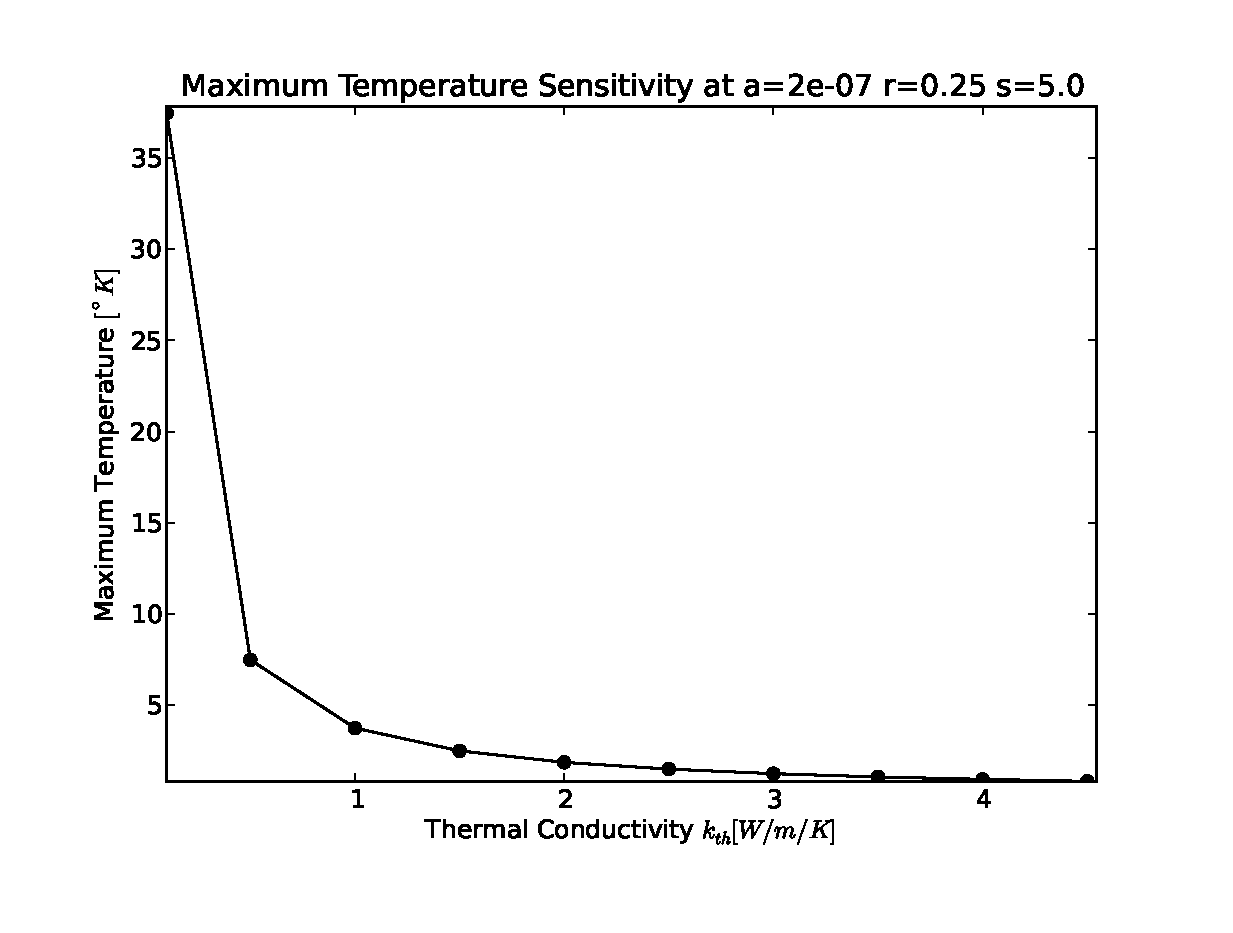
\includegraphics[height=0.7\textheight]{./thermal_demonstration/conductivity/conductivity.eps}
\end{center}
\caption[$K_{th}$ Sensitivity in LLNL Model]{Increased thermal conductivity 
decreases the temperature (here represented by STC) at the limiting radius.}
\label{fig:Cm242Kth_alpha_low}
\end{figure}

\end{frame}


\begin{frame}[ctb!]
\frametitle{Cyder Thermal Conductivity Sensitivity}
\begin{figure}[htbp!]
\begin{center}
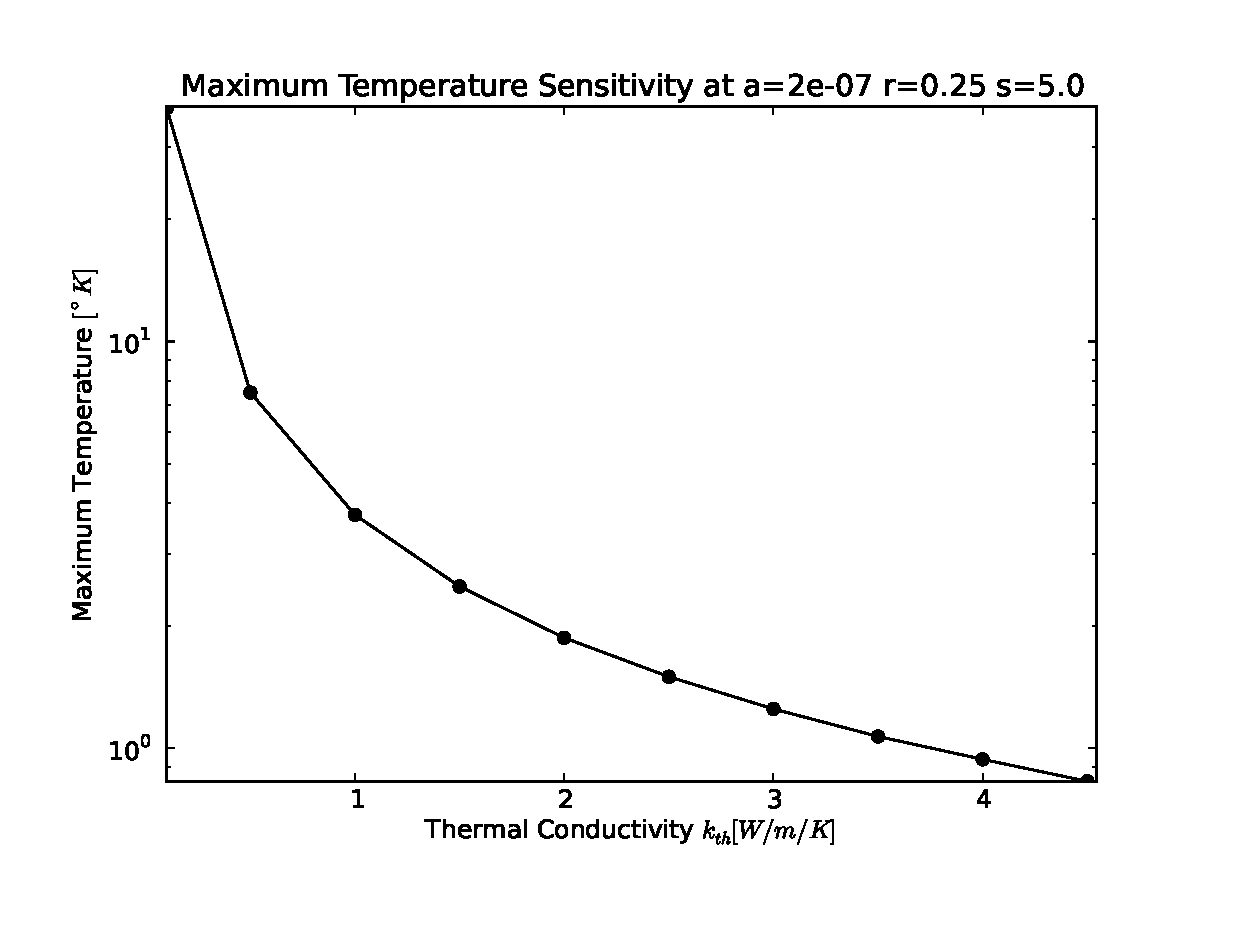
\includegraphics[height=0.7\textheight]{./thermal_demonstration/conductivity/conductivity_cyder.eps}
\end{center}
\caption[$K_{th}$ Sensitivity in Cyder]
{Cyder results agree with those of the LLNL model. Increased $K_{th}$ decreases 
temperature change at the limiting radius. The above example thermal 
profile results from 10kg of $^{242}Cm$, $\alpha_{th}=2\times 10^{-7}$, $s=5m$, 
and $r_{lim}=0.25m$.}
\label{fig:kr}
\end{figure}
\end{frame}

%\begin{frame}[ctb!]
%\frametitle{Cyder Thermal Conductivity and Limiting Radius Sensitivity}
%\begin{figure}[htbp!]
%\begin{center}
%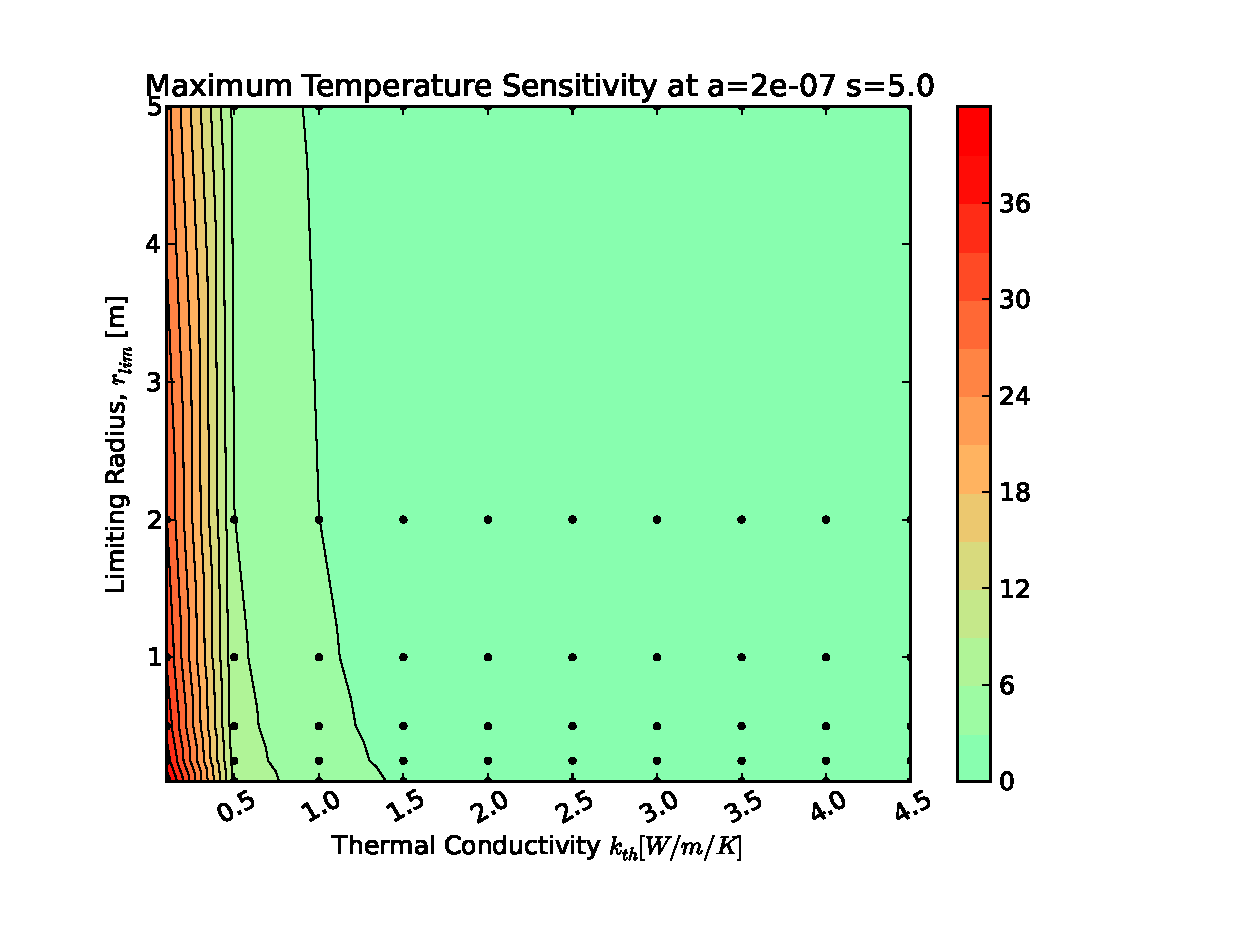
\includegraphics[height=0.7\textheight]{./thermal_demonstration/conductivity/kr.eps}
%\end{center}
%\caption[$K_{th}$ vs. $r_{lim}$ Sensitivity in Cyder]
%{Cyder results agree with 
%those of the LLNL model. The importance of the limiting radius decreases with 
%increased $K_{th}$. The above example thermal profile results from 10kg of 
%$^{242}Cm$}
%\label{fig:kr}
%\end{figure}
%\end{frame}


%\begin{frame}[ctb!]
%\frametitle{Cyder Thermal Conductivity and Limiting Radius Sensitivity}
%\begin{figure}[htbp!]
%\begin{center}
%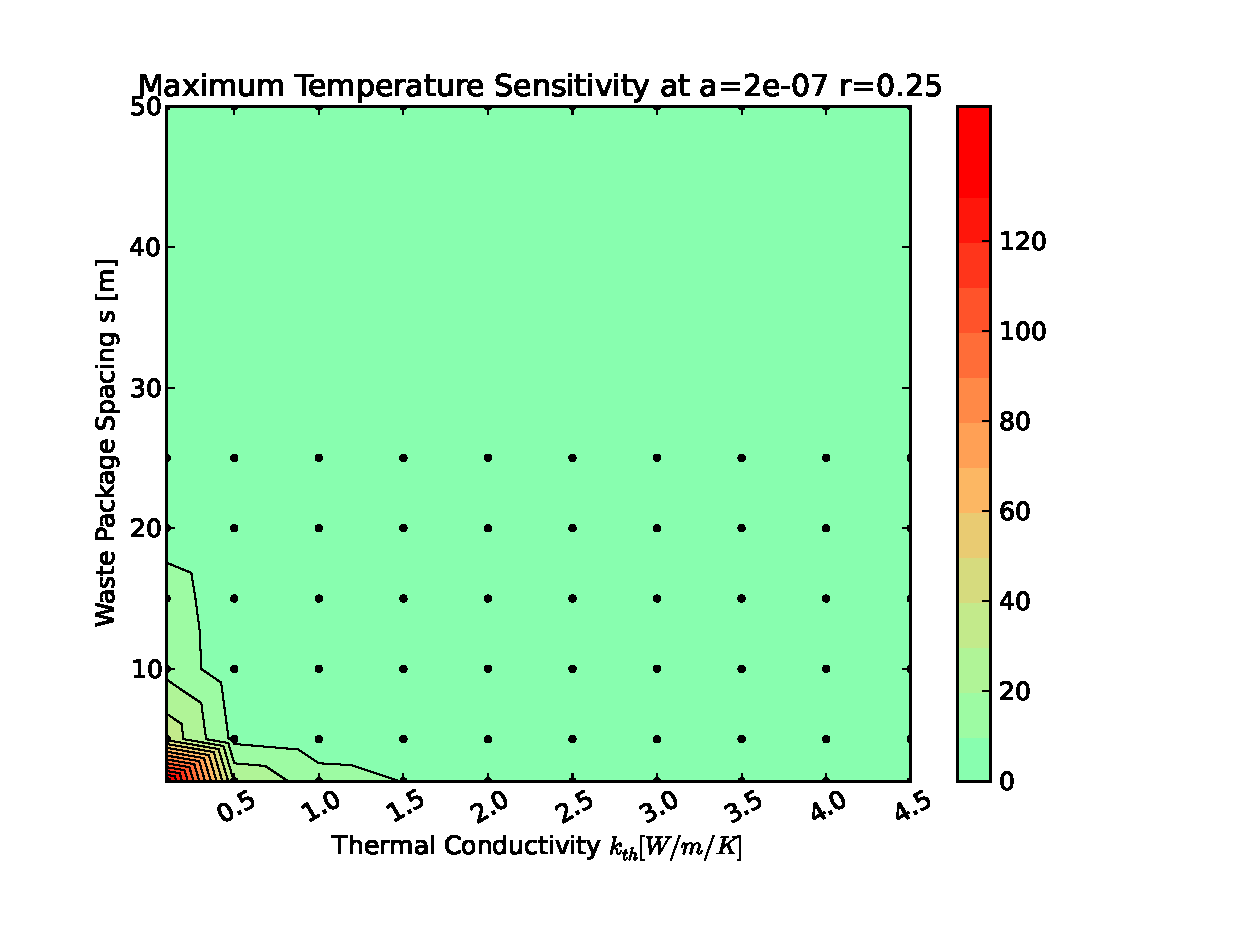
\includegraphics[height=0.7\textheight]{./thermal_demonstration/conductivity/ks.eps}
%\end{center}
%\caption[$K_{th}$ vs. Waste Package Spacing Sensitivity in Cyder]{Cyder results agree with 
%those of the LLNL model. The importance of the limiting radius decreases with 
%increased $K_{th}$. The above example thermal profile results from 10kg of 
%$^{242}Cm$}
%\label{fig:ks}
%\end{figure}
%\end{frame}
